\documentclass[11pt, a4paper]{article}   	% use "amsart" instead of "article" for AMSLaTeX format
\usepackage[margin = 1in]{geometry}                		% See geometry.pdf to learn the layout options. There are lots.
\geometry{letterpaper}                   		% ... or a4paper or a5paper or ... 
%\geometry{landscape}                		% Activate for rotated page geometry
%\usepackage[parfill]{parskip}    		% Activate to begin paragraphs with an empty line rather than an indent
\usepackage{graphicx}				% Use pdf, png, jpg, or eps§ with pdflatex; use eps in DVI mode
								% TeX will automatically convert eps --> pdf in pdflatex		
\usepackage{amssymb}
\usepackage{amsmath}
\usepackage{amsfonts}
\usepackage[utf8]{inputenc}
\usepackage[T1]{fontenc}
\usepackage{caption}

%SetFonts

%SetFonts
\usepackage{titling}
\graphicspath{ {./images/} }
\usepackage{enumitem}	
\usepackage{float}

\setlength{\droptitle}{-8em} 

\title{Group Model}
\author{Team 12}
%\date{}							% Activate to display a given date or no date

\begin{document}
\maketitle
%\subsection{}
\section{Data Analysis}

\begin{figure}[H]\centering
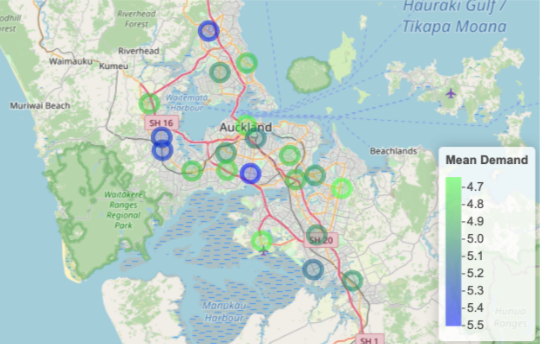
\includegraphics[scale=0.35]{D1}
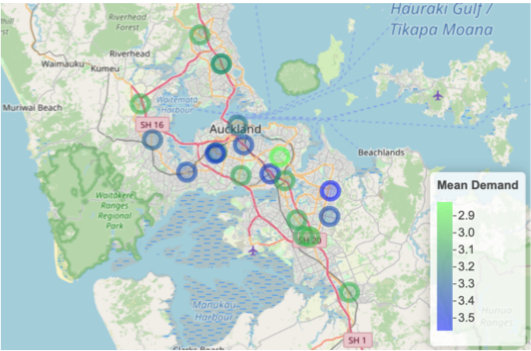
\includegraphics[scale=0.35]{D2}
\caption{\textbf{Mean demand for each of The Warehouse Group stores.}}
\end{figure}

From the figures above we can see that the mean daily pallet demand for both The Warehouse stores and Noel Leeming stores varies by less than 1 pallet per day. Furthermore, there does not appear to be any clear spatial trends in mean daily pallet demand for the different stores. For this reason we will make the assumption that we can characterise the mean daily pallet demand for the stores by store type instead of considering each store individually.

\begin{figure}[H]\centering
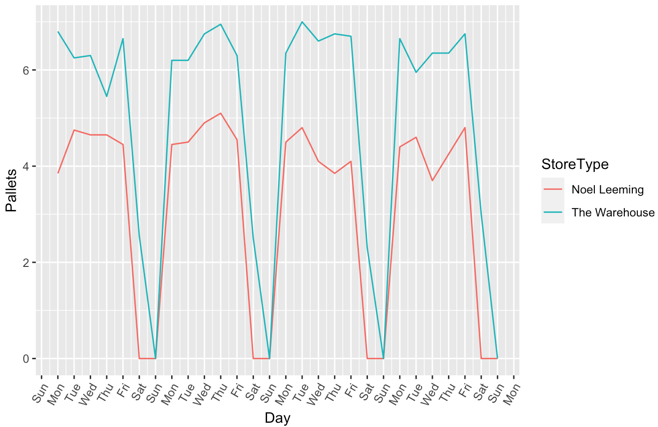
\includegraphics[scale=0.45]{D3}
\caption{\textbf{Mean daily pallet demand for The Warehouse Group Stores from 3rd February to 1st March 2020}}
\end{figure}

\noindent From the plot above it appears that the average daily pallet demand for The Warehouse stores is higher than the Noel Leeming stores. We can also see during the weekdays daily pallet demand seems to be relatively constant for each store type. The average daily pallet demand for The Warehouse stores during the weekdays is around 7 pallets whereas for Noel Leeming stores it is around 5 pallets. The Noel Leeming stores do not appear to have any demand for pallets on the weekend. The Warehouse stores only have pallet demand on Saturday but not Sunday. To investigate the demands on different weekdays we will now create a grouped boxplot.

\begin{figure}[H]\centering
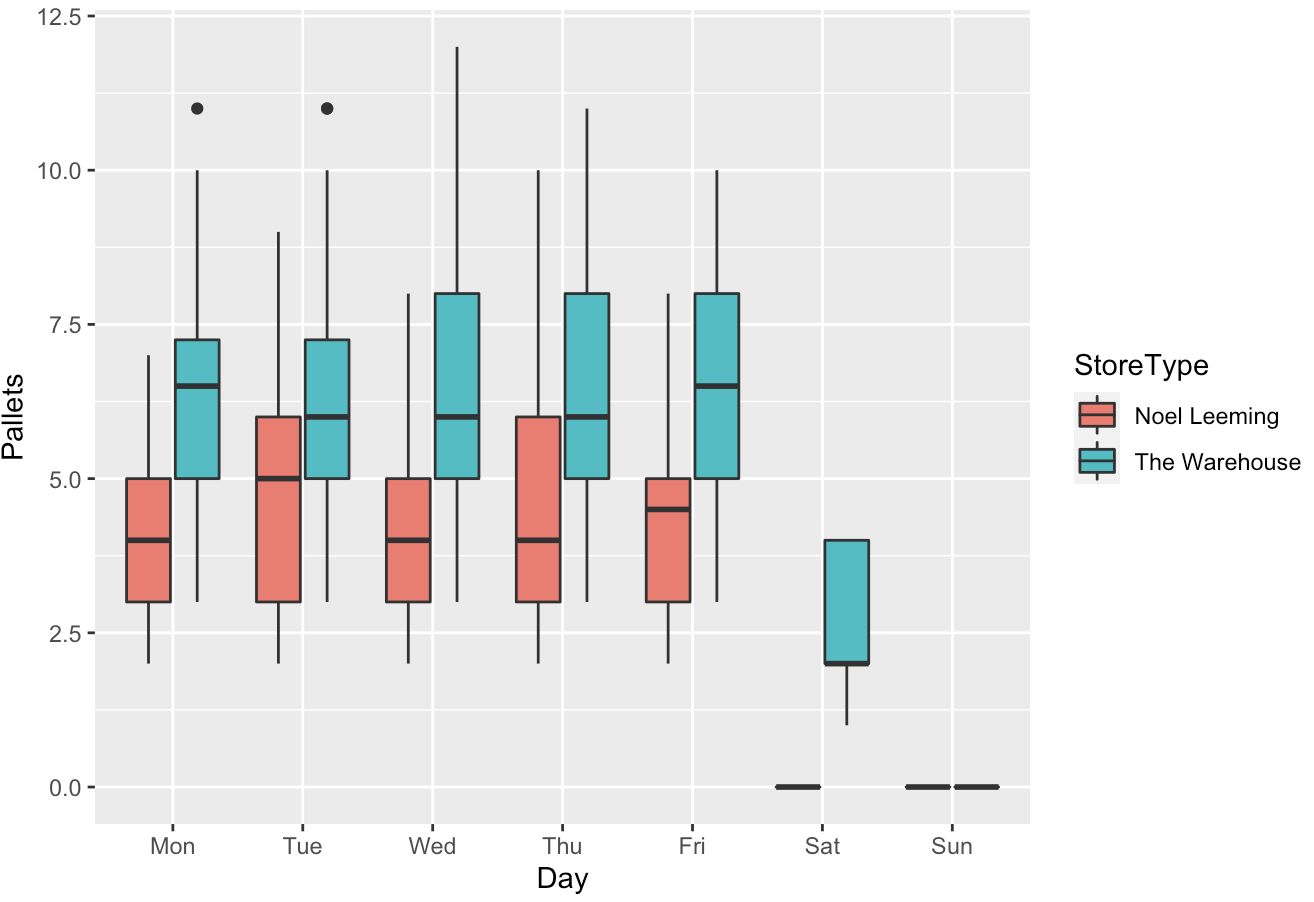
\includegraphics[scale=0.45]{D4}
\caption{\textbf{Daily Pallet demand for The Warehouse Group stores for each day of the week coloured by store type.}}
\end{figure}

\noindent From the boxplot above it would appear an appropriate estimate for daily pallet demand can be made by splitting demand into 3 groups. The groups are as follows; The Warehouse stores during the weekdays, Noel Leeming stores during the weekdays, The Warehouse stores on Saturday. With the daily pallet demand for Noel Leeming stores on the weekend being 0 and the daily pallet demand for The Warehouse on Sunday also being 0. To find a suitable estimate of demand for these different groups we will consider the following violin plots.
\begin{figure}[H]\centering
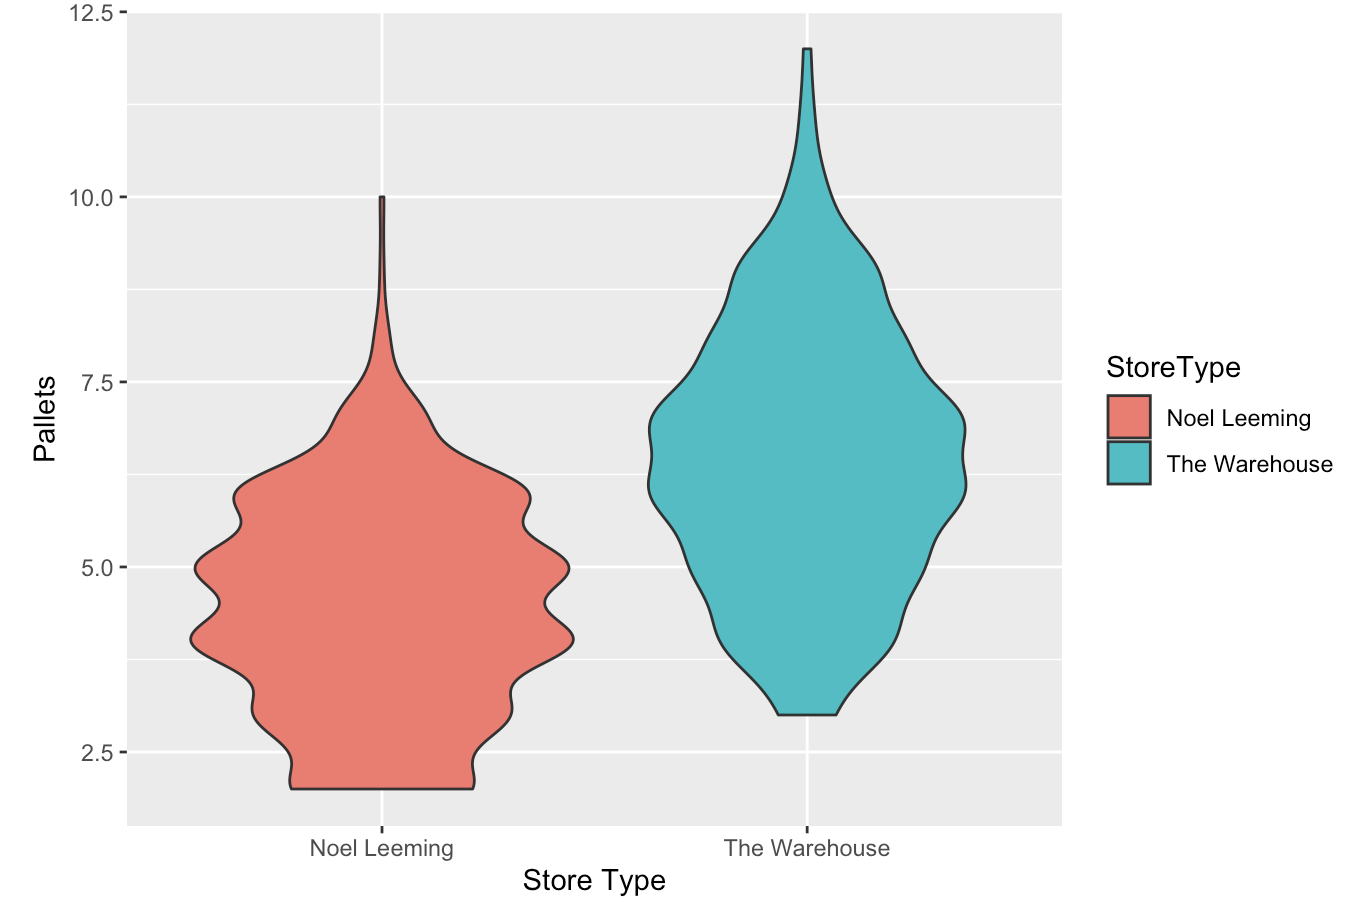
\includegraphics[scale=.3]{D5}
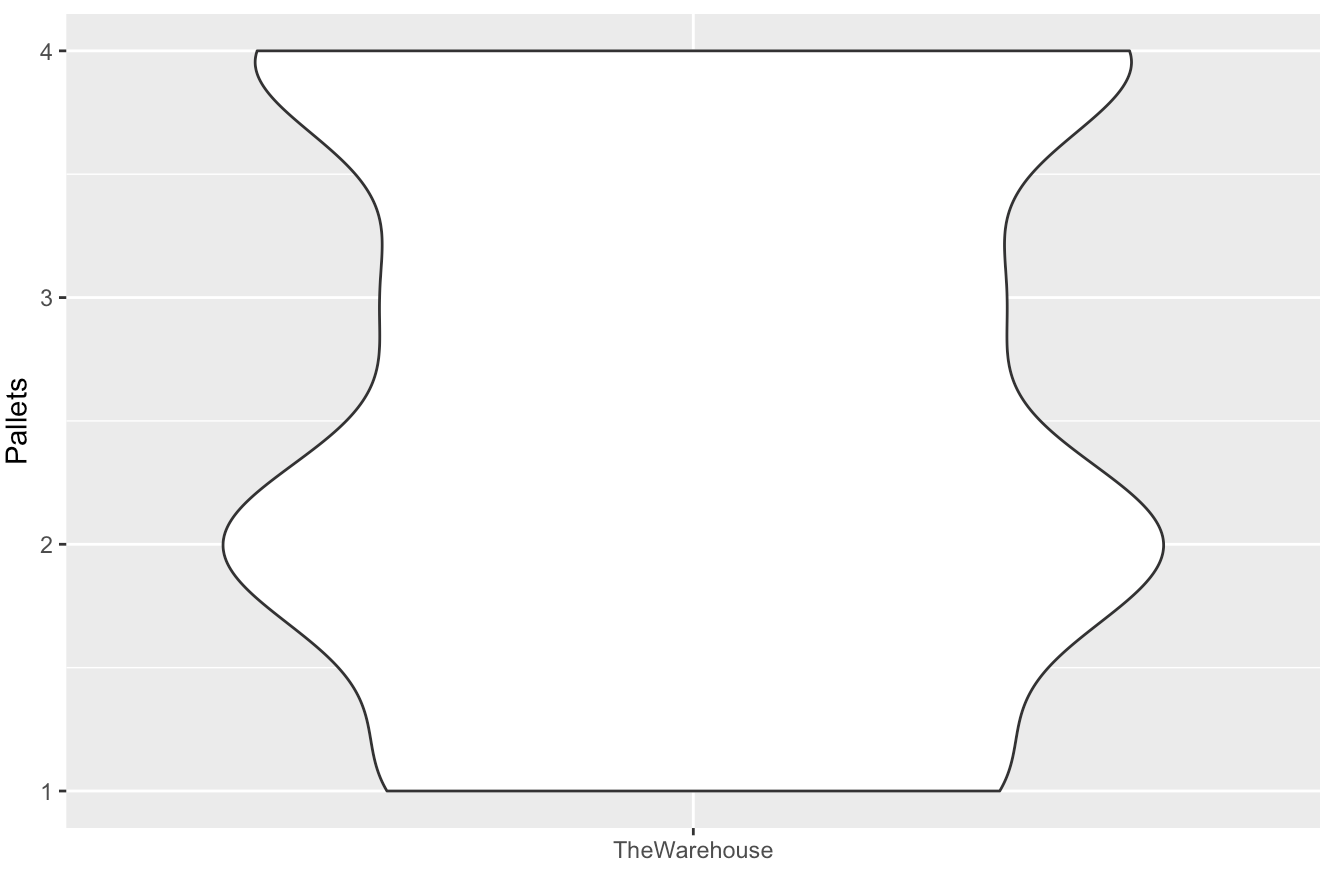
\includegraphics[scale=.3]{D6}
\caption{\textbf{Daily pallet demands for both stores during the weekdays and The Warehouse on Saturday.}}
\end{figure}

\noindent From the violin plots above it appears that a suitable estimate for the daily pallet demand for Noel Leeming stores is 6 pallets per weekday. Similarly a suitable estimate for the daily pallet demand for The Warehouse stores is 8 pallets per day. Finally, we will estimate that the pallet demand for The Warehouse stores on Saturday will be 3 pallets. These estimates around the 75th percentile will ensure that most of the time the trucks will be able to transport enough pallets to satisfy demand of the stores.  \\

\begin{figure}[H]\centering
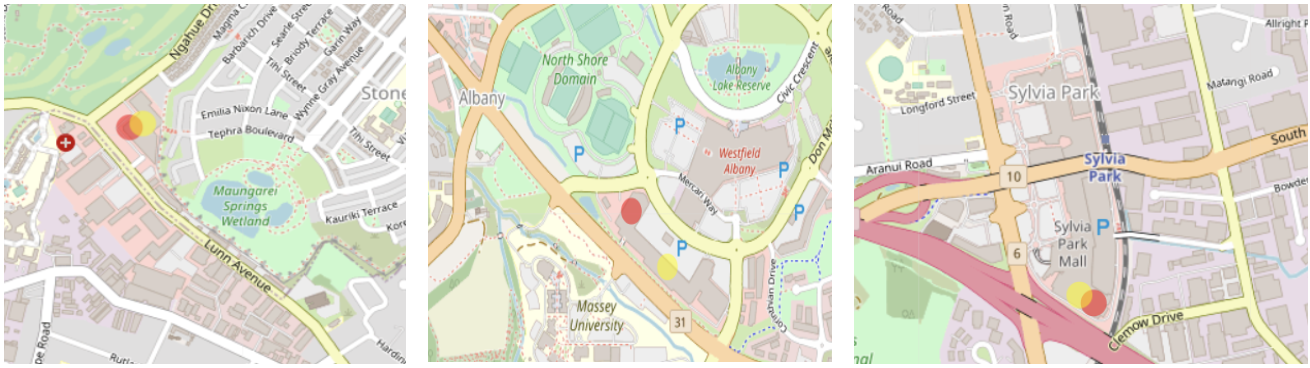
\includegraphics[scale=0.7]{S1}
\caption{\textbf{The Warehouse and Noel Leeming stores that share the same building}}
\end{figure}

\noindent Through the store location visualisations we have decided to group 4 pairs of stores together: The Warehouse and Noel leeming Albany, Lunn Avenue, and Sylvia Park branches, and the Noel Leeming Glenfield clearance and Wairau Park branches. The Albany, Lunn Avenue, and Sylvia Park stores were grouped together because they shared the same building, which can be seen from the figures shown above. Therefore we concluded  that they would also share a loading dock allowing for all pallets to be dropped in the same location. The Noel Leeming Glenfield clearance and Wairau Park branches share the exact same location and therefore it was logical to group the two branches together.


\section{Route Generation}
In order to form and solve the vehicle routing problem we need to construct a set of possible feasible routes. The algorithm we implemented generates feasible routes as follows:

\begin{enumerate}
\item Select a random store as the first store to visit. Set as current store and add to store set for the route.
\item Generate a random number between 2 and 5 that limits the maximum number of stores that will be visited in the route.
\item Continue to add stores to the route until either the maximum number of stores is reached, or the route takes longer than 4 hours.
\item To select the next store, sort stores by distance from the current store then randomly select one of the closest three stores
\item Provided the next store is not already in the route, does not take the route time over 4 hours, and does not exceed truck capacity of 20 pallets add the next store to the store set. If truck capacity or time limit is exceeded break from loop and route is completed.
\item Repeat until a set number of feasible routes is generated (we set this to be 1000).
\end{enumerate}

\noindent We will now discuss the justification of certain aspects of our algorithm. Firstly, we decided to vary the number of stores each route visits by setting a random maximum number of stores. This is to ensure that we have a broad variety of different routes to feed into our linear program. For this reason, we also added the additional random component of selecting one of the 3 closest stores instead of just selecting the closest store.  The \texttt{keep\_looping} condition that stops adding stores to the route (when truck capacity or time limit is reached)  was added to stop the algorithm becoming ‘stuck’. Since it is possible for a set of stores to have a total pallet demand of slightly below 20 (say 17-19) without this break condition the algorithm would continue to try adding a store even if no stores with a pallet demand of 1-3 pallets existed. In this way the algorithm would get stuck in an infinite loop.

\section{Formulation}
In order to formulate and solve the problem, the routes generated from the algorithm described above were put into a standard data structure. The structure used was a dataframe where each route was represented as a column and each row was a different store. The element $ij$ of the matrix was 1 if store $i$ was visited in route $j$ otherwise 0. The cost of each route was stored in a \texttt{Pandas} series with the same indexing as the column names in the dataframe. In order to model the option to ‘wet-lease’ trucks from Mainfreight each route is included in the dataframe twice, with different costs depending on which truck is used. \\

	\noindent 
	The model is formulated using the generalised dataframe and series described above. For simplicity, extra costs caused by traffic won’t be considered in the formulation. However, it will be added to the formulation later on. \\
	
	\noindent
	Let Route$_{i}$ and Route$_{i\text{b}}$ be the binary decisions variables with $\begin{cases}
		1: \text{route chosen}\\
		0: \text{route not chosen}
	\end{cases}$  \\
where Route$_{i}$ are the routes taken by current 25 trucks and Route$_{i\text{b}}$ are the routes taken by `wet-leased' mainfrieght trucks for $i=1,2,3,\dots$. up to the number of generated routes.\\
	
	\noindent 
	Our aim is to minimize the delivery cost which has the objective function of
	\[
	\sum_{i=1}^{n} \text{Route}_{i}\times \text{Cost}_{i} +\sum_{i=1}^{n} \text{Route}_{i\text{b}}\times \text{Cost}_{i\text{b}}
	\] 
	One of the constraints is that all stores are visited exactly once. Mathematically, this can be shown as
	\[
	\sum_{i=1}^{n} \text{Route}_{i}\times \text{store}_{ij}+\sum_{i=1}^{n} \text{Route}_{i\text{b}}\times \text{store}_{ij}=1 \ \text{for} \ j=1,2,3,\dots,N_\text{store}  
	\]
	\[
	\text{with store}_{ij}=\begin{cases} 
	1: \ \text{if store $j$ is in route $i$ / $i$b}\\
	0: \ \text{if store $j$ is not in route $i$  / $i$b} 
	\end{cases}
	\]
	For $N_{\text{store}}$ stores, we have $N_{\text{store}}$ constraints as above. \\
	\newpage
	\noindent  Since we have 25 trucks and they can do 2 shifts each, the maximum number of Route$_i$'s chosen cannot exceed 50. Therefore, we have the final constraint.
	\[
	\sum_{i=1}^{n} \text{Route}_i \leq 50
	\]
	
	
\section{Results}
We then ran the model to get some preliminary results. The table below shows the expected cost of our least-cost routing schedule and the number of truck shifts that are needed.

	\begin{center}
	\begin{tabular}{|c|c|c|}
		\hline
		\textbf{Both Distribution Centres Open} & \textbf{Cost} (\$) & \textbf{Number of Routes} \\
		\hline
		Weekday & 10589.12 & 17 \\
		\hline
		Saturday & 2898.04 & 5 \\
		\hline
		Weekly Total & 55843.64 &  \\
		\hline
		\textbf{Southern Distribution Centre only} &  &  \\
		\hline
		Weekday & 11660.59 & 18 \\
		\hline
		Saturday & 3124.08 & 5 \\
		\hline
		Weekly Total & 61427.03 &  \\
		\hline
	\end{tabular}
	\captionof{table}{Preliminary results}
	\end{center}

\noindent From our initial results it is clear that operating 25 trucks is more than sufficient to ensure that the total pallet demand can be met at The Warehouse Group stores even when the Northern distribution centre is closed. We can conclude The Warehouse Group would not need to invest in additional trucks in the event the Northern distribution centre is closed.  \\ 

\noindent We also found that the additional cost to deliver the pallets if the Northern distribution centre is closed is approximately \$5580 per week. This equates to approximately \$24,300 per month. Since closing the Northern Distribution centre will save \$400,000 per month it appears that this is the recommended course of action. But more work will need to be done to investigate the wider implications of closing the Northern distribution centre. In particular, how does this impact the resilience and overall efficiency of the delivery system.



\end{document}  